\documentclass{llncs}
\usepackage[T1]{fontenc}
\usepackage{graphicx}
\usepackage{enumitem}
\usepackage{amsmath}
\usepackage{listings}
\usepackage{tikz}
\usepackage{epstopdf}
\usepackage{multirow}
\usepackage{todonotes}

\title{Evaluating the Effectiveness of AEX-Notify against SGX Single-Stepping Attackers}
\author{Wicked Wench}
\institute{	University of L\"ubeck, Germany}
% TODO: For the camera-ready submission
%\author{Basil Ugbomoiko\inst{1} \quad Daniel Knaack\inst{1}}
%\institute{	University of L\"ubeck, Germany\\
%	\email{\{basil.ugbomoiko,daniel.knaack\}@student.uni-luebeck.de}}

\begin{document}

\maketitle

\begin{abstract}
  Trusted execution environments (TEEs) like Intel's Software Guard Extensions (SGX)
  offer a promising avenue for securing applications by executing them within secure enclaves.
  However, recent advancements in side-channel attack techniques, such as SGX-Step,
  pose significant threats to the security guarantees provided by SGX.
  SGX-Step uses the APIC timer to precisely interrupt the enclave after each instruction,
  effectively stepping through the execution one instruction at a time.
  These single-stepping capabilities allow much greater granularity for side-channel,
  thereby enhancing the feasibility of side-channel attacks.
  In response to this threat, AEX-Notify has been proposed as a potential mitigation against SGX-Step.
  AEX-Notify is both a hardware extension and a software mitigation that tries
  to prevent adversaries from single-stepping enclaves.
  This paper analyzes the security of AEX-Notify and evaluates its
  effectiveness against deterministic single-stepping.
\end{abstract}

\section{Motivation}

Modern computing relies heavily on privileged system software to manage interactions and ensure security.
However, traditional operating system kernels are susceptible to bugs and vulnerabilities
due to their large codebase written in unsafe languages.
To address this, recent research has focused on Protected Module Architectures (PMAs),
aiming to support isolated execution of security-sensitive components
called enclaves with minimal Trusted Computing Base (TCB).
Intel’s Software Guard eXtensions (SGX) \cite{Intel16,Intel17} represent a significant advancement,
providing hardware-enforced trusted computing guarantees.
However, vulnerabilities have emerged, particularly in information leakage
through attacks exploiting various system components.
These vulnerabilities undermine the security promises of SGX.

SGX-Step presents a novel framework to address SGX vulnerabilities by enabling
precise monitoring of enclave execution at the instruction level.
Unlike previous methods, SGX-Step achieves true single-stepping for any enclave program,
significantly enhancing the resolution of existing attacks.
The framework comprises a Linux kernel driver and a runtime library,
providing the means to interrupt enclave execution at the instruction level
for detailed observation and analysis.

\paragraph{Introduction to AEX-Notify}
\begin{itemize}
  \item Overview of AEX-Notify
  \item Potential benefits of using AEX-Notify
\end{itemize}

For Intel SGX enclaves, AEX-Notify is a security feature that prevents single-stepping attacks such as SGX-Step. Enclaves can react to possible threats by using the ability to recognize Asynchronous Enclave eXit (AEX) events \cite{ConstableBCXXAK23}.

A notification mechanism for AEX events is added by AEX-Notify. In order to stop data leaking or control flow manipulation, the enclave can take defensive measures, such as deleting sensitive data or resetting execution states, when an AEX happens \cite{ConstableBCXXAK23}.

The primary advantage of AEX-Notify is its capacity to improve enclave security by the detection of AEX events, which interferes with the timing required for attacks. By enabling enclaves to confirm their current state upon restart and apply adaptive security measures, it contributes to the maintenance of execution integrity by boosting resilience against a variety of interruption-based threats \cite{ConstableBCXXAK23}.

\paragraph{Research Question and Objectives}
\begin{itemize}
  \item Formulation of the \textbf{research question}:
    Is it possible to gather control-flow information of victim programs running
    in SGX enclaves when the victim protects the execution of the enclave with
    AEX-Notify?
  \item \textbf{Project goals}:
    Our goal is to evaluate the effectiveness of AEX-Notify against SGX-step by
    constructing an example program where the SGX-Step attack works and testing
    this program once with AEX-Notify enabled and once without. We will compare
    the results to see how much information we can gain about control-flow
    information with and without AEX-Notify enabled.
\end{itemize}

\section{Background}

This section provides a comprehensive review of existing research and frameworks
relevant to the evaluation of AEX-Notify against SGX single-stepping attackers.
In particular, we outline the workings of Intel SGX and
discuss how SGX-Step leverages the APIC timer to single-step enclaves.
Following this, we examine CopyCat, which leverages SGX-Step to extract
control-flow information from enclaves, highlighting potential security
vulnerabilities.
Finally, we look into the details of AEX-Notify and
how it prevents the single-stepping capabilities of SGX-Step.

/section{Intel SGX}
The security feature that allows for the construction of safe enclaves within applications is introduced by Intel Software Guard Extensions (SGX) \cite{CostanD16}. Sensitive code and data are placed in protected execution environments known as enclaves, which guarantee confidentiality and integrity even in the event that the host system is compromised.

The strong memory management system of SGX is one of its core features. In order to effectively prevent unwanted access to enclave data, SGX imposes rigorous memory segregation between enclaves and non-enclave programs.

Moreover, SGX offers exception and interrupt management techniques. An Asynchronous Enclave eXit (AEX) is initiated in response to an interrupt, maintaining the state of the program in the active Saved State Area (SSA). However, enclave programs lack an interrupt detection mechanism in the absence of supplementary measures such as AEX-Notify.

SGX defines key constructs including the Thread Control Structure (TCS) and Saved State Area (SSA) to control enclave execution and state transitions. The current stored state area within the TCS is specifically indicated by the \texttt{TCS.CSSA}.

In addition, SGX instructions such as EENTER and EEXIT help to maintain the integrity of the enclave's execution environment by facilitating a safe transfer of control flow between enclave and non-enclave code.

It is important to note that SGX does not by itself offer protection against side-channel attacks, even if its primary goal is to safeguard the integrity and confidentiality of enclave data and code. It is the duty of developers to incorporate extra precautions to lessen these dangers in their enclave implementations \cite{CostanD16}.
\subsection{SGX-Step}
SGX-Step \cite{BulckPS17} is a framework that enhances the ability to monitor SGX enclave execution at the instruction level, addressing vulnerabilities by enabling precise and detailed observation. It uses the APIC timer to interrupt enclave execution at specific intervals, overcoming previous challenges related to time jitter by configuring the timer in user space for finer control and reduced jitter \cite{ArnautovTGKMPLM16}.

The monitoring of Page Table Entries (PTEs) is one of SGX-Step's primary features. Even if single-stepping enclave execution is quite sluggish, it can be used for certain functions alone. Single-stepping can begin using SGX-Step once a specific code or data page is accessed \cite{BulckWKPS17}. It configures mappings between user space virtual memory and the physical memory that houses the PTEs in the enclave. Using the "present" bit to cause page faults \cite{XuCP15} or the "accessed" and "dirty" properties to reveal information about how much memory is being used in the enclave, an attacker can manipulate these PTEs.

All things considered, side-channel attacks are made far more likely by SGX-Step's accurate interrupt control and PTE monitoring, which give adversaries access to critical information at the instruction level as well as comprehensive control flow information \cite{BulckPS17}.

\begin{figure}[t]
  \centering
  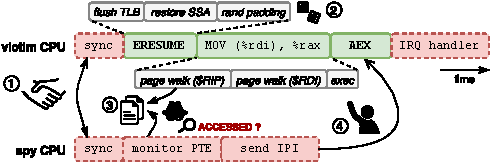
\includegraphics{images/sgx-step-pte.pdf}
  \caption{Overview of the SGX-Step attack.
    After resuming execution, the enclave has to lookup the pages for
    the instruction itself and the \texttt{rdi} operand. This increases the time
    for the instruction and therefore the likelihood that an interrupts arrives
    during the execution of that instruction.}
  \label{fig:sgx-step-pte}
\end{figure}

\todo[inline]{Add paragraph for monitoring page table entries and how SGX-Step
  uses it to start single-stepping once a specific page has been executed.}
Enabling side-channel attacks depends on SGX-Step's ability to precisely halt enclave execution. Attackers can learn about the control flow and data usage patterns inside the enclave by looking at the execution flow at such a fine level. This thorough observation emphasizes the necessity of strong defenses against such assaults by showing how vulnerabilities can be exploited and sensitive data extracted.

\todo[inline]{Explain why SGX-Step is important $\to$ It enables side-channel attacks at instruction-level granularity}
The importance of SGX-Step is seen in its potential to facilitate side-channel attacks within Intel SGX enclaves at the instruction level. Using the APIC timer to generate precise interrupts, SGX-Step makes it possible to observe enclave execution in detail. Attackers can now more accurately detect vulnerabilities, take advantage of timing side-channels, and extract sensitive data. By giving attackers precise control over enclave execution, SGX-Step essentially increases the attack surface and is a potent weapon for breaking into SGX-protected apps.
\subsection{CopyCat}

CopyCat \cite{MoghimiBHPS20} utilizes the SGX-Step framework
to infer fine-grained control-flow information from SGX enclaves.
It improves upon traditional page-fault adversaries,
that can only page accesses at a 4 KiB resolution,
with the single-stepping capabilities of SGX-Step.

\begin{figure}[t]
  \centering
  \includegraphics{square-and-multiply.pdf}
  \caption{A typical implementation of the exponentiation function using square and multiply.
    The function calculates $c^d$ where $c$ and $d$ are natural numbers.
    It is important to note that \emph{square} and \emph{multiply} are separate functions
    and may reside on different pages than the exponentiation function.}
  \label{fig:square-and-multiply}
\end{figure}

In a typical square-and-multiply implementation,
we can use page faults to extract the key.
On each iteration we can induce a fault by clearing the execute permission on
the page with the \emph{square} function.
Tracking access in each iteration, we can fully recover the key from only page faults.

Traditional page-fault adversaries fail at recovering the key when the entire
square-and-multiply procedure fits on a single page.
CopyCat overcomes this challenge by single-stepping the enclave and counting the
number of instructions until a data page was accessed.
By comparing the data access pattern with the function, CopyCat is able to recover the key
even if all used functions fit on a single page.

Figure~\ref{fig:square-and-multiply} illustrates the square-and-multiply example.
There are two data accesses of interest.
The first is the access to the output message $m$ that is squared on each iteration.
The second is the access to the cipher text when we multiply $m$ by $c$.
This data access only happens when the key bit $d[i]$ equals one.
Hence, we will have three data accesses to $c$, $m$ and $d$ in one iteration,
while we will have only two accesses if the key bit is zero.
Therefore, by counting the number of instructions in each iteration,
CopyCat can recover the key even if the cipher text, output and key are on the same page.

%\todo[inline]{Add paragraph explaining why this is a problem in the context of
%  the SGX attacker model. Because technically side-channel attacks are not a
%  concern for SGX, but they still implemented AEX-Notify.}

\subsection{AEX-Notify}
\label{sec:aex-notify}

To counter SGX-Step and the attack vectors that it enables, AEX-Notify has been proposed.
The purpose of AEX-Notify is to stop attackers from reliably single-stepping an enclave,
which mitigates many attacks based on SGX-Step like CopyCat.

Constable et al. \cite{ConstableBCXXAK23} list the main reason
behind the effectiveness of SGX-Step as the assisted page-table walk.
Before resuming the enclave, the attacker clears
the ``accessed'' (A) bit on the enclave's code page.
This forces the first instruction after \texttt{ERESUME}
to perform an expensive microcode assist to set the A-bit.
This induces additional latency in the execution of that instruction, because
the processor has to walk the page table again.
Thus, there is a large time frame where the interrupt of the timer could
arrive and land exactly on the first instruction.
The goal of AEX-Notify is to reduce the latency of the first instruction
and make it impossible to reliably land on the first instruction.

\paragraph{Hardware Extension.}
The first part of AEX-Notify is the hardware extension.
It introduces a new flag in the SSA frame, called \texttt{AEXNOTIFY}.
By enabling this flag, we change the behavior of the \texttt{ERESUME} instruction.
Usually, \texttt{ERESUME} restores the previous process context,
however, when the \texttt{AEXNOTIFY} bit is enabled,
a custom exception handler is executed.
The exception handler is responsible for handling the AEX and
can resume the enclave application with an additional instruction, called \texttt{EDECCSSA}.
This instruction decrements \texttt{TCS.CSSA} and restores the context of the enclave application.

\paragraph{Software Mitigation.}
The second part of AEX-Notify is the custom exception handler that is implemented in software.
The exception handler is split into two stages.
The first stage is responsible for decoding the first instruction and
computing the accessed pages of that instruction.
It is run with \texttt{AEXNOTIFY} disabled.
The second stage is responsible for prefetching the addresses from the first stage.
It is further split into two parts.
The first part runs with \texttt{AEXNOTIFY} disabled
and the second, smaller assembly stub runs with \texttt{AEXNOTIFY} enabled.
AEX-Notify is disabled at first to ensure that the exception handler always makes forward progress.

\section{Work Description}

Our main goal is to analyze the effectiveness of AEX-Notify
in preventing attackers from reliably single-stepping SGX enclaves.
To evaluate the success of AEX-Notify,
we conducted an analysis aimed at identifying any potential weak points in its implementation.
This section outlines the steps we took in our evaluation process,
beginning with the setup of the SGX-Step attack and
the subsequent enabling of AEX-Notify on this attacker.
By examining these components,
we aimed to provide an informed assessment of AEX-Notify’s defensive capabilities.
This analysis has informed us about potential attack vectors to try,
offering insights into areas that may require further study.

\iffalse
  \subsection{Experimental Setup}

  Since AEX-Notify consists of a hardware and software part,
  we need a system that specifically supports the hardware extension.
  This section outlines the hardware and software specifications of the experimental environment,
  including configuration details necessary for conducting the evaluation.

  \textbf{Hardware and Software Specifications:}
  \begin{itemize}
    \item Intel Core i7 10th Gen, 16GB DDR4 RAM, and SSD storage.
    \item Ubuntu 20.04 LTS (Linux kernel version 5.10) with SGX driver support. Use SGX SDK for enclave development.
  \end{itemize}

  \textbf{Configuration Details:}
  \begin{itemize}
    \item
      Configure SGX environment with appropriate BIOS settings and SGX driver installation.
      Utilize SGX SDK for enclave development.
    \item
      Set up the environment to execute the single-stepping attack.
      Select target enclaves and configure attack parameters for testing.
  \end{itemize}
\fi

\subsection{Attacker Model}

In this project, we assume the standard Intel SGX privileged attacker model.
This means that the attacker has full control over the operating system
and can control important system functions.
For example, the attacker may modify the page-table to learn about memory accesses
or they may configure the APIC timer to interrupt the enclave, like SGX-Step.
This model is particularly relevant in scenarios such as cloud computing
environments, where cloud service providers could potentially exploit their
privileged access to the hardware and software stack to launch attacks against SGX enclaves.

\subsection{Initializing SGX-Step}

%\todo[inline]{Explain kernel module, \texttt{/dev/sgx-step}, etc.}

SGX-Step requires careful configuration of the APIC timer
since it is crucial for the attack to work.
If the value is too small, then we will zero-step and execute the same instruction multiple times.
If the value is too large, then we will multi-step and execute multiple instructions.
We have used the benchmark application provided in the SGX-Step repository for this purpose.
The program consists only of a series of \texttt{nop} instructions and
reports the instruction pointer after each interrupt using the \texttt{EDBGRD} instruction.
If the instruction pointer is incremented by one instruction each interrupt,
then we can be sure that we are single-stepping and
that we have configured SGX-Step correctly.

\subsection{Enabling AEX-Notify}

After configuring SGX-Step and successfully single-stepping the enclave,
we enabled AEX-Notify.
We have enabled AEX-Notify by simply adding an additional field in the enclave configuration file.
Enabling this flag technically requires registering an exception handler that handles any enclave exits.
However, the exception handler is preconfigured to use the provided handler
from the trusted runtime system of the Intel SGX SDK.
This is the exact same exception handler as described in Section~\ref{sec:aex-notify},
which decodes the enclave return point and prefetches the necessary code and data pages.

\subsection{Analyzing AEX-Notify}

After enabling AEX-Notify, we verified that we can no longer single-step the enclave
by comparing the reported addresses from a previous run.
Usually, we can use these addresses to configure the timer
since each address is incremented by one when the timer is configured correctly.
The problem with AEX-Notify is that interrupting the enclave not only
interrupts the enclave but it can also interrupt the exception handler.
Hence, the application will additionally report addresses from the exception handler.

For these addresses, it is not entirely clear where exactly there are from.
Therefore, we have written a simple tool that uses the debug information from the binary and
automatically translates these addresses to their source code location in the trusted runtime system.

%\todo[inline]{Explain how we analyzed AEX-Notify, i.e. comparing the source with the reported addresses.}

The overall analysis has lead us to an important question regarding the exception handler:
whether interrupting the exception handler during the second stage would
restart the entire exception handler again or only restart the second stage.
If an interrupt during the second stage would only restart the second stage,
then we could effectively differentiate between a zero and a multi-step.

We have analyzed this potential weak point by modifying the second stage to cause an interrupt.
This involved adding one additional instruction in the second stage.
This instruction would access a page that the enclave has no read permission for.
Hence, a page fault occurs and the enclave is interrupted during the second stage.
The last step is recognizing where this interrupt is handled.
To achieve this, we induce another page fault on the first stage of the exception handler
and we check whether another page fault occurs immediately after the first.

\section{Results}

\paragraph{Single-Stepping Resilience.}
As the most basic requirement,
we were no longer able to single-step the enclave after enabling AEX-Notify.
We were always able to reliably interrupt the application
before executing the first instruction of the target code
by using the additional page-fault side channel provided by SGX-Step.
However, we were unable to reliably execute one or
even multiple instructions after executing the first.

The reason was that we were no longer just interrupting the enclave but also the exception handler of AEX-Notify.
Since the application reports the instruction pointer of the enclave,
we could see that the addresses no longer correspond to only our target.
Instead, most of these addresses pointed to the exception handler.
Between these addresses, sometimes the program would report addresses from our target.
However, the addresses always jumped at least several instructions from the previous
and we were never able to reliably cause a controlled multi-step attack
by only configuring the APIC timer.

% TODO: Report about C3 Cache

\paragraph{Interrupting the Exception Handler.}
We were able to verify that the exception handler is always rolled back to the first phase of the exception handler
even if the handler itself is interrupted.
By inserting a page-fault after the assembly stub re-enables AEX-Notify,
we were able to detect that the exception handler is reset completely,
i.e. it starts from the first phase.
This ensures that an attacker cannot simply interrupt the exception handler
to differentiate between a zero-step and a multi-step,
showing the security of AEX-Notify.

\section{Conclusion and Future Work}

With this study, we explored the functionality of AEX-Notify in Intel SGX and
its effectiveness in preventing single-stepping attacks.
Our experiments showed that once AEX-Notify is enabled,
single-stepping attacks are no longer feasible,
indicating that AEX-Notify is effective in stopping such attacks.

In conclusion, our findings suggest that AEX-Notify is a promising feature for enhancing SGX security,
but additional testing is necessary to confirm its effectiveness against a wider range of attacks.

\bibliographystyle{alpha}
%\bibliographystyle{splncs03}
\bibliography{references}
\end{document}
